\documentclass[documentclass]{jsarticle}
\usepackage[top=25truemm,bottom=25truemm,left=20truemm,right=20truemm]{geometry}
\usepackage{listings, jlisting, color}
\usepackage[dvipdfmx]{graphicx}
\usepackage{pdfpages}
\usepackage{amsmath}
\usepackage{amssymb, latexsym}
\usepackage{mathtools}
\usepackage{multirow}
\usepackage{color}
\usepackage{ulem}
\usepackage{here}
\usepackage{wrapfig}
\usepackage{tikz}
\usepackage{color}
\usepackage{url}
\usetikzlibrary{intersections, calc, arrows, positioning, arrows.meta}


\newcommand{\Add}[1]{\textcolor{red}{#1}}
\newcommand{\Erase}[1]{\textcolor{red}{\sout{\textcolor{black}{#1}}}}
\newcommand{\ctext}[1]{\raise0.2ex\hbox{\textcircled{\scriptsize{#1}}}}
\newcommand{\red}[1]{\textcolor{red}{#1}}

\lstset{
  basicstyle=\ttfamily,
  %basicstyle={\small},
  breaklines=true,
  frame=single,
  tabsize=3,
  numbers=left
}

\begin{document}
\title{情報理論 第14回 計算機演習}
\author{222C1021 今村優希}
\maketitle

\newpage

\section*{演習1}
\subsection*{演習1-1}
IMのASCIIコードを符号化する.

\begin{itemize}
  \item I : 0100 1001
  \item M : 0100 1101
\end{itemize}

(7,4)ハミング符号なので,4bitずつ符号化を行う.
また,検査ビットを式\ref*{sq:1-1}と設定する.
\begin{equation}
  \left\{ \,
    \begin{aligned}
      &c_1 = a_1 \oplus a_2 \oplus a_3 \\
      &c_2 = a_2 \oplus a_3 \oplus a_4 \\
      &c_3 = a_1 \oplus a_2 \oplus a_4 
    \end{aligned}
  \right.
  \label{sq:1-1}
\end{equation}

\paragraph*{0100の符号化}
式\ref*{sq:1-1}を利用して$c_1$から$c_3$まで求めると,
\begin{align*}
  c_1 = 1, c_2 = 1, c_3 = 1
\end{align*}
と検査ビットを計算できる.したがって,送信符号は(0100111)である.

\paragraph*{1001の符号化}
式\ref*{sq:1-1}を利用して,
\begin{align*}
  c_1 = 1, c_2 = 1, c_3 = 0
\end{align*}
と計算ビット計算できる.したがって,送信符号は(1001110)である.

\paragraph*{0100の符号化}
式\ref*{sq:1-1}を利用して,
\begin{align*}
  c_1 = 1, c_2 = 1, c_3 = 1
\end{align*}
と検査ビットが計算できる.したがって,送信符号は(0100111)である.

\paragraph*{1101の符号化}
式\ref*{sq:1-1}を利用して,
\begin{align*}
  c_1 = 0, c_2 = 0, c_3 = 1
\end{align*}
と検査ビット計算できる.したがって,送信符号は(1101001)である.

以上から,送信される符号は,(0100111 1001110 0100111 1101001)となる.

\subsection*{演習1-2}
自分の学籍番号の下一桁+1番目と11番目のbitに誤りが発生すると仮定するので,受信符号は
\begin{center}
  (0\red{0}00111 100\red{0}110 0100111 1101001)
\end{center}
である.誤りが発生した部分を赤文字で表している.
\newpage

また,シーケンスは
\begin{equation}
  \left\{ \,
    \begin{aligned}
      &s_1 = a_1 \oplus a_2 \oplus a_3 \oplus c_1\\
      &s_2 = a_2 \oplus a_3 \oplus a_4 \oplus c_2\\
      &s_3 = a_1 \oplus a_2 \oplus a_4 \oplus c_3
    \end{aligned}
  \right.
  \label{sq:1-2}
\end{equation}
で計算できる.
このシーケンスから得られるエラーテーブルを表\ref*{tb:1-1}に表す.
\begin{table}[H]
  \begin{center}
    \caption{エラーテーブル}
    \label{tb:1-1}
    \begin{tabular}{|ccccccc|c|} \hline
     $e_1$ & $e_2$ & $e_3$ & $e_4$ & $e_5$ & $e_6$ & $e_7$ & $s_1 s_2 s_3$ \\ \hline
     0 & 0 & 0 & 0 & 0 & 0 & 0 & 000 \\ 
     1 & 0 & 0 & 0 & 0 & 0 & 0 & 101 \\ 
     0 & 1 & 0 & 0 & 0 & 0 & 0 & 111 \\ 
     0 & 0 & 1 & 0 & 0 & 0 & 0 & 110 \\ 
     0 & 0 & 0 & 1 & 0 & 0 & 0 & 011 \\ 
     0 & 0 & 0 & 0 & 1 & 0 & 0 & 100 \\ 
     0 & 0 & 0 & 0 & 0 & 1 & 0 & 010 \\ 
     0 & 0 & 0 & 0 & 0 & 0 & 1 & 001 \\ \hline
    \end{tabular}
  \end{center}
\end{table}

\paragraph*{0000111の復号化}
式\ref*{sq:1-2}を利用して,得られるシーケンスは,
\begin{align*}
  s_1 = 1, s_2 = 1, s_3 = 1
\end{align*}
である.エラーテーブルから2bit目が誤りだと分かるので訂正して,(0100)が正しい符号である.

\paragraph*{1000110の復号化}
式\ref*{sq:1-2}を利用して,得られるシーケンスは,
\begin{align*}
  s_0 = 1, s_2 = 1, s_3 = 1
\end{align*}
である.エラーテーブルから4bit目が誤りだと分かるので訂正して,(1001)が正しい符号である.

\paragraph*{0100111 と 1101001の復号化}
式\ref*{sq:1-2}を利用して,得られるシーケンスは,0100111と1101001どちらも
\begin{align*}
  s_1 = 0, s_2 = 0, s_3 = 0
\end{align*}
である.シーケンスがすべて0ではないので正しく受信できている.
したがって,(0100)と(1101)が受信符号である.

よって,復号化して得られる符号は,(0100 1001 0100 1101)である.

\subsection*{演習1-3}
今回は復号化がうまくできた場合である.

ハミング(7,4)符号は,1bitの誤りまで訂正することが可能である.
今回の誤り場所は1つの符号に1つしかないので,ハミング(7,4)符号で誤り訂正が可能であった.
逆に,誤り訂正ができない場合は,1つの符号に2つの誤りが発生した時である.
2つ誤りが発生した場合は,誤りの検出は可能だが,誤った場所を特定することができない.


\newpage

\section*{演習2}
\subsection*{演習2-1}
BSCの相互情報量$I(X;Y)$の計算を行う.$P_X(0)=r$とし,誤り率は$p$で表現する.
% BSCの状態を以下のfigureで表現できそうだったら行う.
\begin{figure}[H]
  \begin{center}
    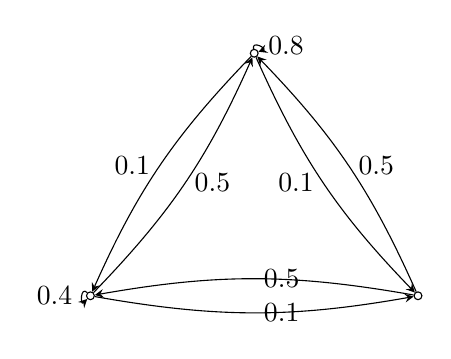
\begin{tikzpicture}[node/.style={draw, circle, font=\small, inner sep=1pt}]
      \node[node](s1) {};
      \node[node, below left = 3cm and 2cm of s1](s2) {};
      \node[node, below right  = 3cm and 2cm of s1](s3) {};
  
      \path[->, >=stealth]
        (s1) edge[loop right, in=20, out=100, looseness=4] node{0.8} (s1)
        (s1) edge[left, bend right=10] node{0.1} (s2)
        (s1) edge[left, bend right=10] node{0.1} (s3)
        (s2) edge[right, bend right=10] node{0.5} (s1)
        (s2) edge[loop left, in=225, out=135, looseness=4] node{0.4} (s2)
        (s2) edge[right, bend right=10] node{0.1} (s3)
        (s3) edge[right, bend right=10] node{0.5} (s1)
        (s3) edge[right, bend right=10] node{0.5} (s2);
    \end{tikzpicture}
  \end{center}
  \caption{状態遷移図}
  \label{fig:2-1}
\end{figure}

まずは,結合確率を求める.
\begin{align}
  P_{X,Y}(0,0) &= r(1-p) \\ \label{sq:1-3}
  P_{X,Y}(0,1) &= rp \\
  P_{X,Y}(1,0) &= (1-r)p \\
  P_{X,Y}(1,1) &= (1-r)(1-p) 
\end{align}
それから,周辺確率を求めると,
\begin{align}
  P_X(0) &= r \\ 
  P_X(1) &= 1-r\\
  P_Y(0) &= P_{X,Y}(0,0) + P_{X,Y}(1,0) = r(1-p) + (1-r)p\\
  P_Y(1) &= P_{X,Y}(0,1) + P_{X,Y}(1,1) = rp + (1-r)(1-p) \label{sq:1-4}
\end{align}
となる.式\ref*{sq:1-3}から\ref*{sq:1-4}を用いて条件付き確率を求める.
\begin{align}
  P_{X|Y}(0|0) = \dfrac{P_{X,Y}(0,0)}{P_Y(0)} = \dfrac{r(1-p)}{r(1-p) + (1-r)p} \\
  P_{X|Y}(1|0) = \dfrac{P_{X,Y}(1,0)}{P_Y(0)} = \dfrac{(1-r)p}{r(1-p) + (1-r)p} \\
  P_{X|Y}(0|1) = \dfrac{P_{X,Y}(0,1)}{P_Y(1)} = \dfrac{rp}{rp + (1-r)(1-p)} \\
  P_{X|Y}(1|1) = \dfrac{P_{X,Y}(1,1)}{P_Y(1)} = \dfrac{(1-r)(1-p)}{rp + (1-r)(1-p)} \label{sq:1-7}
\end{align}
次に条件付きエントロピーを求める.条件付きエントロピーは,
\begin{align}
  H(X|Y) &=P_Y(0)H(X|Y=0) + P_Y(1)H(X|Y=1)\\
  \begin{split}
    & = P_Y(0)\big(-P_{X|Y}(0|0) \log_2{P_{X|Y}(0|0)} -P_{X|Y}(1|0) \log_2{P_{X|Y}(1|0)}\big)\\
    & \qquad + P_Y(1)\big(-P_{X|Y}(0|1) \log_2{P_{X|Y}(0|1)} -P_{X|Y}(1|1) \log_2{P_{X|Y}(1|1)}\big) 
  \end{split}
  \\
  \begin{split}
    &= - P_{X,Y}(0,0)\log_2{P_{X|Y}(0|0)} - -P_{X,Y}(1,0)\log_2{P_{X|Y}(1|0)} \\
    & \qquad - P_{X,Y}(0,1)\log_2{P_{X|Y}(0|1)} - -P_{X,Y}(1,1)\log_2{P_{X|Y}(1|1)} \label{sq:1-6}
  \end{split}
\end{align}
と変形できる.
式\ref*{sq:1-6}に,式\ref*{sq:1-3}から\ref*{sq:1-7}を代入していくと,条件付きエントロピー$H(X|Y)$は,
\begin{align}
  \begin{split}
    H(X|Y) &= -r(1-p) \log_2 \dfrac{r(1-p)}{r(1-p) + (1-r)p} - \big(r(1-p) + (1-r)p\big) \log_2 \dfrac{rp}{rp + (1-r)(1-p)}  \\
    & \qquad - rp \log_2 \dfrac{(1-r)p}{r(1-p) + (1-r)p} - \big(rp + (1-r)(1-p)\big) \log_2 \dfrac{(1-r)(1-p)}{rp + (1-r)(1-p)}
  \end{split}
\end{align}
となる.さらに,事前エントロピー$H(X)$は,
\begin{align}
  H(X) = -r \log_2 r - (1-r) \log_2 (1-r)
\end{align}
で求めることができる.したがって,相互情報量$I(X;Y)$は,
\begin{align}
  I(X;Y) &= H(X) - H(X|Y)\\
  \begin{split}
    &= -r \log_2 r - (1-r) \log_2 (1-r)\\
    & \qquad-\Big(-r(1-p) \log_2 \dfrac{r(1-p)}{r(1-p) + (1-r)p} - \big(r(1-p) + (1-r)p\big) \log_2 \dfrac{rp}{rp + (1-r)(1-p)}  \\
    & \qquad \quad - rp \log_2 \dfrac{(1-r)p}{r(1-p) + (1-r)p} - \big(rp + (1-r)(1-p)\big) \log_2 \dfrac{(1-r)(1-p)}{rp + (1-r)(1-p)}\Big)
  \end{split}
  \\
  &= p \log_2{p} + (1-p) \log_2{(1-p)} - (r+p-2rp) \log_2{(r+p-2rp)} - (1-r-p+2rp) \log_2{(1-r-p+2rp)} \label{sq:1-8}
\end{align}
と算出することができる.教科書等では$H_f(p)$などとまとめていたが,続く設問のプログラムで式\ref*{sq:1-8}を直接使用するのでまとめる行為は行わなかった.

\subsection*{演習2-2}
$r = \dfrac{1}{2}$としたときの$I(X;Y)$と$p$の関係のグラフをMatlabで作成する.
まず,演習2-1で算出した$I(X;Y)$に対して,$r = \dfrac{1}{2}$を代入すると,
\begin{align}
  H(X;Y) = 1 + p \log_2{p} + (1-p) \log_2{(1-p)}
\end{align}
となるので,この式を利用してMatlabでプログラムの作成を行った.
ソースコード\ref*{sc:2-1}では,xをエラー確率として,0から1まで0.001刻みで遷移させている.
最後にその値をグラフにプロットしたものが図\ref*{fig:2-2}である.
横軸がエラー確率,縦軸が相互情報量を表している.

%ソースコード挿入
\lstinputlisting[caption=エラー確率と相互情報量の関係のプログラム \label{sc:2-1}]{code/ensyuu2_2.m}

\begin{figure}[H]
  \begin{center}
    \includegraphics*[]{figure/2-1.png}
  \end{center}
  \caption{エラー確率と相互情報量の関係}
  \label{fig:2-2}
\end{figure}


\subsection*{演習2-3}
演習2-2から,通信路容量の最大値を求める.
通信路容量は,
\begin{align}
  C = \max{I(X;Y)} = \max{\{H(X) - H(X|Y)\}}
\end{align}
で求めることができる.
したがって,\ref*{fig:2-2}のグラフから見ると,$C = \max_{P(X)}I(X;Y)$は,$p=1,0$のときに最大値の1を取ることがわかる.
よって,通信路容量の最大値は1である.
\subsection*{演習2-4}
Matlabを用いて$r = \dfrac{1}{2}$となる情報源を作成し,BSCを通過させるようなプログラムを作成し,その結果について考察を行った.

\subsubsection*{プログラム}
作成したプログラムは,ソースコード\ref*{sc:2-2}である.
このプログラムで情報源の発生,BSCの通過から相互情報量の値を出力することができる.

プログラムの流れに関して説明をする.
15行目から送信符号を生成し,BSCに通過させている.
送信するビット数が100,000bitなので1から100,00までfor文を回している.
16行目でxに0から100まで整数の乱数を発生させている.18行目以降のif文ないで,生成された値を2のmodを取ることで送信符号の0,1を作っている.
乱数なので,このとき$r = \dfrac{1}{2}$であると考える.
次に,確率用の0から1以下の乱数を生成させている.
この乱数が設定しているエラー確率より大きいか小さいかを判断することでBSCを通過のモデルを実現している.
35行目以降は,相互情報量を求めるために,結合確率や周辺確率,条件付きエントロピーの計算を行っている.
このプログラムのフローチャートを図\ref*{fig:2-3}で示している.

%ソースコード挿入
\lstinputlisting[caption=BSC通過プログラム \label{sc:2-2}]{code/ensyuu2_4.m}

\begin{figure}[H]
  \begin{center}
    \includegraphics*[scale=0.25]{figure/2-2.jpg}
  \end{center}
  \caption{プログラムのフローチャート}
  \label{fig:2-3}
\end{figure}


\subsubsection*{出力結果}
以下のソースコード\ref*{sc:2-3}から\ref*{sc:2-4}はエラー確率を0.2, 0.5, 0.8のとき結果である.

%ソースコード挿入
\lstinputlisting[caption=エラー確率0.2のときの実行結果\label{sc:2-3}]{code/result-ensyuu2_4-p0.2.txt}
\lstinputlisting[caption=エラー確率0.5のときの実行結果]{code/result-ensyuu2_4-p0.5.txt}
\lstinputlisting[caption=エラー確率0.8のときの実行結果\label{sc:2-4}]{code/result-ensyuu2_4-p0.8.txt}

\subsubsection*{考察}
上記の結果から,BSCに通した場合,エラー確率が$\dfrac{1}{2}$のときに相互情報量が小さくなることがわかる.
エラー確率が0.5のとき,0が0に,0が1に,1が0に,1が1になる回数がほぼ同じであった.
よって,事前の情報と事後の情報の相互依存していないことがわかる.
一方,エラー確率が0や1に近かった場合,相互情報量が大きいので相互依存していると考えられる.

また,今回,送信信号を出力する部分からの作成を行った.
エラー確率によって相互情報量が数式\ref*{sq:1-8}のように変化している.
この変化を確認するために,ソースコード\ref*{sc:2-2}を一部変更して,エラー確率ごとの相互情報量を出力してグラフを出力するプログラムを作成した.
このプログラムを実行した結果が図\ref*{fig:2-3}である.
このグラフの近似曲線は,演習2-2で作成したグラフとほとんど同じである.
よって,作成したプログラムはBSCを忠実に再現しているモデルだと考えることができる.

\begin{figure}[H]
  \begin{center}
    \includegraphics*[]{figure/2-3.png}
  \end{center}
  \caption{エラー確率と相互情報量の関係}
  \label{fig:2-3}
\end{figure}
\newpage

\section*{演習3}
\subsection*{演習3-1}
素数同士の積$pq$から,素数$p$,$q$を導き出すプログラムの作成を行った.
プログラム自体はpythonを用いて行い,実行時間の出力まで一貫して行うプログラムを作成した.
ソースコードは\ref*{sc:3-1}である.
このプログラムでは,iを2からpqまでfor文で増加させている.
pqがiで割れたとき,pqの素数のうち1つがiであることから,pにiを挿入することで素数を求めている.
qはpqを求めたpで割ることで必然的に求めることができる.

プログラムを実行して得られた結果は,
\begin{align*}
  pq &= 323  → \qquad p = 17, \qquad q = 19\\
  pq &= 110489 → \qquad p = 313, \qquad q = 353\\
  pq &= 4295229443 → \qquad p = 65537, \qquad = 65539\\
  pq &= 1082249732248967 → \qquad p =  12346793, \qquad q = 87654319
\end{align*}
である.

%ソースコード挿入
\lstinputlisting[caption=素数を導き出すプログラム\label{sc:3-1}]{code/ensyuu3-1.py}



\subsection*{演習3-2}
演習3-1で使用した$pq = 4295229443$と$pq = 1082249732248967$のときの$p$と$q$を求めるのにかかる時間を計測する.
自分の環境は,
\begin{itemize}
  \item CPU: Intel(R) Core(TM) i7-1195G7
  \item コア数: 4
  \item クロック周波数: 2.90GHz
  \item メモリ容量: 16.0GB
\end{itemize}
である.
実行結果を以下のソースコード\ref*{sc:3-2}で示している.
$p=4295229443$のときの実行時間は0.0057214秒である.
また,$1082249732248967$のときの実行時間は,1.0662479であった.

%ソースコード挿入
\lstinputlisting[caption=実行時間の計測\label{sc:3-2}]{code/result-ensyuu3_2.txt}

\subsection*{演習3-3}
パラメータを$p=7, q=11$に設定し,RSA暗号で0b001101 010011を暗号化,復号を行う.
\begin{align}
  (p-1)(q-1) = 6 \times 10 = 60
\end{align}
これと互いに素となる$e$として13に設定する.
\begin{align}
&13 \cdot d \equiv 1(\mod60)\\
&13 \times 37 = 481 \equiv 1(\mod60)
\end{align}
よって,公開鍵を$(e,n)=(13,77)$,秘密鍵を$(d)=(37)$となる.

また,10進数77以下でないと暗号化できないので,6bitを1つの値として暗号化を行う.
\begin{itemize}
  \item 0b001101 = 0d13
  \item 0b010011 = 0d19
\end{itemize}
より,暗号化は
\begin{align}
  C_1 = 13^{13} \mod 77 = 41\\
  C_2 = 19^{13} \mod 77 = 61
\end{align}
となる.また,暗号化したものを復号すると,
\begin{align}
  P_1 = 41^{37} \mod 77 = 13\\
  P_2 = 61^{37} \mod 77 = 19
\end{align}
と求めることができる.

\newpage

\subsection*{今回使用したプログラム}
今回使用したプログラムを以下にアップロードした.

\url{https://github.com/tanusai646/information-theory-for-matlab}
\end{document}